\section{Graphs}

A graph\idx{Graph} is a structure that can be used to model how things relate to each other. Graphs consists of nodes\idx{Node} (also called vertices) and edges\idx{Edge} between them. There are many variations over the theme, but the most basic one is the \textsl{undirected}\idxx{Graph!Undirected}{Undirected} graph. It can be defined as:
\begin{eqnarray*}
  G = (N,E)
\end{eqnarray*}
Here, $N$ is the set of nodes and $E$ is the set of edges. We often choose to illustrate nodes as circles or boxes, and edges as lines.

% edges: directionality
Edges can have a more complex role in graphs. The most common complexity is for the edges to be directed\idxx{Edge!Directed}{Directed edge}. That is, the edge is has a \textsl{source}\idx{Source node} node, and a \textsl{destination}\idx{Destination node} node. Depending on the graph type, these may be the same node. Graphs with directed edges are called \textsl{directed}\idxx{Graph!Directed}{Directed graph}. Formally, we have:
\begin{eqnarray*}
  E \subseteq \{ (s,d) \mid (s,d) \in N^2 \}
\end{eqnarray*}
% edges: weight
Another common complexity is to associate edges with \textsl{weights}\idxx{Edge!Weight}{Edge weight}. A weight is, at its core, a number. Graphs with weighted edges are called \textsl{Weighted}\idxx{Graph!Weighted}{Weighted graph}. Usually, it represents a cost. An example of a directed weighted graph can be seen in figure \ref{fig:topics:graphs:example:base}.

\begin{figure}[tbp]
  \begin{center}
    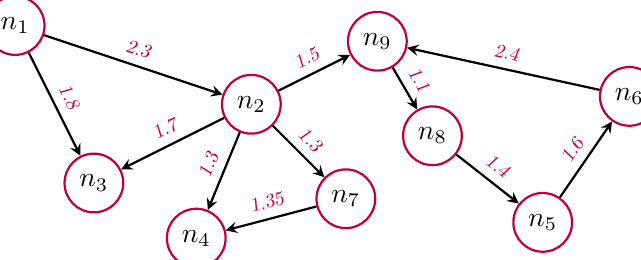
\begin{tikzpicture}[remember picture]
      \newcommand{\weight}[1]{node[midway,sloped,above] {\scalebox{0.7}{\textsl{\textcolor{purple}{#1}}}}}
      \tikzstyle{edge}  = [thick,>=stealth,draw=black]
      \tikzstyle{dedge} = [thick,->,>=stealth,draw=black]
      \tikzstyle{node}=[
        overlay,
        circle,
        draw=purple,
        anchor=center,
        thick,
        minimum size=1,
      ]
      
      \node[node] (n1) at (-4,0) {$n_1$};
      \node[node] (n2) at (-1,-1) {$n_2$};
      \node[node] (n3) at (-3,-2) {$n_3$};
      \node[node] (n4) at (-1.7,-2.7) {$n_4$};
      \node[node] (n5) at (2.7,-2.5) {$n_5$};
      \node[node] (n6) at (3.8,-0.9) {$n_6$};
      \node[node] (n7) at (0.2,-2.2) {$n_7$};
      \node[node] (n8) at (1.3,-1.4) {$n_8$};
      \node[node] (n9) at (0.6,-0.2) {$n_9$};
      
      \draw[dedge] (n1)--(n2) \weight{2.3};
      \draw[dedge] (n2)--(n3) \weight{1.7};
      \draw[dedge] (n1)--(n3) \weight{1.8};
      \draw[dedge] (n2)--(n4) \weight{1.3};
      \draw[dedge] (n2)--(n9) \weight{1.5};
      \draw[dedge] (n9)--(n8) \weight{1.1};
      \draw[dedge] (n6)--(n9) \weight{2.4};
      \draw[dedge] (n5)--(n6) \weight{1.6};
      \draw[dedge] (n2)--(n7) \weight{1.3};
      \draw[dedge] (n7)--(n4) \weight{1.35};
      \draw[dedge] (n8)--(n5) \weight{1.4};
    \end{tikzpicture}
  \end{center}
  \caption{Example of directed graph with weighted edges.}
  \label{fig:topics:graphs:example:base}
\end{figure}

\subsection{Paths}

\begin{figure}[tbp]
  \begin{center}
    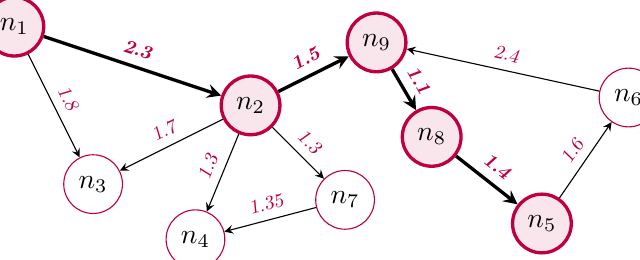
\begin{tikzpicture}[remember picture]
      \newcommand{\weight}[1]{node[midway,sloped,above] {\scalebox{0.7}{\textsl{\textcolor{purple}{#1}}}}}
      \tikzstyle{edge}  = [>=stealth,draw=black]
      \tikzstyle{dedge} = [->,>=stealth,draw=black]
      \tikzstyle{node}=[
        overlay,
        circle,
        draw=purple,
        anchor=center,
        minimum size=1,
      ]
      
      \node[node, very thick, fill=purple!10] (n1) at (-4,0) {$n_1$};
      \node[node, very thick, fill=purple!10] (n2) at (-1,-1) {$n_2$};
      \node[node] (n3) at (-3,-2) {$n_3$};
      \node[node] (n4) at (-1.7,-2.7) {$n_4$};
      \node[node, very thick, fill=purple!10] (n5) at (2.7,-2.5) {$n_5$};
      \node[node] (n6) at (3.8,-0.9) {$n_6$};
      \node[node] (n7) at (0.2,-2.2) {$n_7$};
      \node[node, very thick, fill=purple!10] (n8) at (1.3,-1.4) {$n_8$};
      \node[node, very thick, fill=purple!10] (n9) at (0.6,-0.2) {$n_9$};
      
      \draw[dedge, very thick] (n1)--(n2) \weight{\textbf{2.3}};
      \draw[dedge] (n2)--(n3) \weight{1.7};
      \draw[dedge] (n1)--(n3) \weight{1.8};
      \draw[dedge] (n2)--(n4) \weight{1.3};
      \draw[dedge, very thick] (n2)--(n9) \weight{\textbf{1.5}};
      \draw[dedge, very thick] (n9)--(n8) \weight{\textbf{1.1}};
      \draw[dedge] (n6)--(n9) \weight{2.4};
      \draw[dedge] (n5)--(n6) \weight{1.6};
      \draw[dedge] (n2)--(n7) \weight{1.3};
      \draw[dedge] (n7)--(n4) \weight{1.35};
      \draw[dedge, very thick] (n8)--(n5) \weight{\textbf{1.4}};
    \end{tikzpicture}
  \end{center}
  \caption[Example of a path in a directed graph.]{Example of a path in a directed graph. The path starts in $n_1$, goes through nodes $n_2$, $n_9$, $n_8$ to end in $n_5$. It has a total length of 6.3.}
  \label{fig:topics:graphs:example:path}
\end{figure}

\subsection{Cycles}

\begin{figure}[tbp]
  \begin{center}
    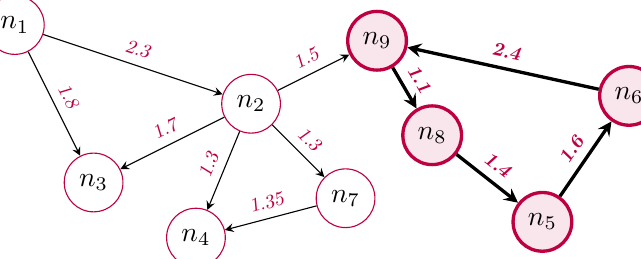
\begin{tikzpicture}[remember picture]
      \newcommand{\weight}[1]{node[midway,sloped,above] {\scalebox{0.7}{\textsl{\textcolor{purple}{#1}}}}}
      \tikzstyle{edge}  = [>=stealth,draw=black]
      \tikzstyle{dedge} = [->,>=stealth,draw=black]
      \tikzstyle{node}=[
        overlay,
        circle,
        draw=purple,
        anchor=center,
        minimum size=1,
      ]
      
      \node[node] (n1) at (-4,0) {$n_1$};
      \node[node] (n2) at (-1,-1) {$n_2$};
      \node[node] (n3) at (-3,-2) {$n_3$};
      \node[node] (n4) at (-1.7,-2.7) {$n_4$};
      \node[node, very thick, fill=purple!10] (n5) at (2.7,-2.5) {$n_5$};
      \node[node, very thick, fill=purple!10] (n6) at (3.8,-0.9) {$n_6$};
      \node[node] (n7) at (0.2,-2.2) {$n_7$};
      \node[node, very thick, fill=purple!10] (n8) at (1.3,-1.4) {$n_8$};
      \node[node, very thick, fill=purple!10] (n9) at (0.6,-0.2) {$n_9$};
      
      \draw[dedge] (n1)--(n2) \weight{2.3};
      \draw[dedge] (n2)--(n3) \weight{1.7};
      \draw[dedge] (n1)--(n3) \weight{1.8};
      \draw[dedge] (n2)--(n4) \weight{1.3};
      \draw[dedge] (n2)--(n9) \weight{1.5};
      \draw[dedge, very thick] (n9)--(n8) \weight{\textbf{1.1}};
      \draw[dedge, very thick] (n6)--(n9) \weight{\textbf{2.4}};
      \draw[dedge, very thick] (n5)--(n6) \weight{\textbf{1.6}};
      \draw[dedge] (n2)--(n7) \weight{1.3};
      \draw[dedge] (n7)--(n4) \weight{1.35};
      \draw[dedge, very thick] (n8)--(n5) \weight{\textbf{1.4}};
    \end{tikzpicture}
  \end{center}
  \caption[Example of a cycle in a directed graph.]{Example of a cycle in a directed graph. It goes through nodes $n_9$, $n_8$, $n_5$, and $n_6$.}
  \label{fig:topics:graphs:example:cycle}
\end{figure}

\subsection{Directed Acyclic Graphs}

Directed acyclic graphs\idx{DAG}, or DAGs, are directed graphs without cycles. For algorithmic reasons, this is a very attractive quality in a graph.

\subsection{Trees}

% basics
A tree\idx{Tree} is a graph where any pair of nodes are connected by exactly one path. Technically, trees, are undirected graphs. However, most real-world examples are directed graphs where a \textsl{root}\idxx{Tree!Root node}{Root node} node is anchoring the tree. From this node a single path leads to each of the other nodes. These are either called \textsl{leaf}\idxx{Tree!Leaf node}{Leaf node} nodes -- if they have no outgoing edges -- or \textsl{branch}\idxx{Tree!Branch node}{Branch node} nodes. These are typically drawn with the root at the top and leaves at the bottom. That is, growing downwards as shown in figure \ref{fig:topics:graphs:example:tree}. But sometimes, for practical reasons, they are drawn growing towards the right.

\begin{figure}[tbp]
  \begin{center}
    \begin{tikzpicture}[remember picture]
      \newcommand{\unit}[0]{8mm}
      
      \tikzstyle{dedge} = [thick,->,>=stealth,draw=black]
      \tikzstyle{node}=[
        overlay,
        circle,
        thick,
        anchor=center,
        minimum size=1,
      ]
      \tikzstyle{root}=[
        node,
        draw=blue
      ]
      \tikzstyle{branch}=[
        node,
        draw=purple
      ]
      \tikzstyle{leaf}=[
        node,
        draw=teal
      ]
      
      \node[leaf]   (n1111) at (0,0) {};
      \node[leaf]   (n1112) at ([xshift=\unit] n1111) {};
      \node[leaf]   (n1131) at ([xshift=2.5*\unit] n1111) {};
      \node[leaf]   (n1321) at ([xshift=4.5*\unit] n1111) {};
      \node[leaf]   (n1322) at ([xshift=5.5*\unit] n1111) {};
      
      \node[branch] (n111) at ([yshift=\unit] $(n1111)!0.5!(n1112)$) {};
      \node[branch] (n113) at ([yshift=\unit] n1131) {};
      \node[leaf]   (n112) at ($(n111)!0.5!(n113)$) {};
      \node[leaf]   (n131) at ([xshift=-\unit, yshift=\unit] n1321) {};
      \node[branch] (n132) at ([yshift=\unit] $(n1321)!0.5!(n1322)$) {};
      
      \node[branch] (n11) at ([yshift=\unit] $(n111)!0.5!(n113)$) {};
      \node[branch] (n13) at ([yshift=\unit] $(n131)!0.5!(n132)$) {};
      \node[leaf]   (n12) at ($(n11)!0.5!(n13)$) {};
      
      \node[root]   (n1) at ([yshift=\unit] $(n11)!0.5!(n13)$) {};
      
      \draw[dedge] (n1)--(n11);
      \draw[dedge] (n1)--(n12);
      \draw[dedge] (n1)--(n13);
      
      \draw[dedge] (n11)--(n111);
      \draw[dedge] (n11)--(n112);
      \draw[dedge] (n11)--(n113);
      \draw[dedge] (n13)--(n131);
      \draw[dedge] (n13)--(n132);
      
      \draw[dedge] (n111)--(n1111);
      \draw[dedge] (n111)--(n1112);
      \draw[dedge] (n113)--(n1131);
      \draw[dedge] (n132)--(n1321);
      \draw[dedge] (n132)--(n1322);
    \end{tikzpicture}
  \end{center}
  \caption[Example of a tree.]{Example of a tree, with a blue node for the root, a brown node for the branch nodes and green nodes for the leaf nodes.}
  \label{fig:topics:graphs:example:tree}
\end{figure}

% properties: balanced, red-black, binary, B-trees, B+-trees

% forests
Some graphs are simply a number of disconnected tree structures. These are referred to as forests\idx{Forest}.

\subsection{Connectedness}

\subsection{Reachability}

\subsection{Representation}
\subsubsection{Marshalling}

Graphs can be stored in many formats, but one of the more common ones is the DOT\footnote{ \url{https://en.wikipedia.org/wiki/DOT_\%28graph_description_language\%29} } file format.

\subsubsection{Datastructures}

\subsection{Property Graphs}

\subsection{Visual Layout}

\subsection{Use Cases}

\begin{itemize}
  \descitem{Filesystem}
  \descitem{GIT}
  \descitem{User Interfaces}
  \descitem{Dependency Modeling}
  \descitem{HTML/XML}
  \descitem{Route Planning}
  \descitem{Code Optimization}
  \descitem{Searching}
\end{itemize}

